\documentclass[border=4pt]{standalone}
\usepackage[T1]{fontenc}
\usepackage{helvet}
\renewcommand{\familydefault}{\sfdefault}
\usepackage{graphicx}
\usepackage{caption}
\usepackage{amsmath}
\captionsetup{font={sf,footnotesize},labelfont={sf,bf,footnotesize},justification=justified,singlelinecheck=false}
\begin{document}
\setcounter{figure}{4}
\begin{minipage}{7.20in}
\centering
\begin{figure}[htbp]
    \centering
    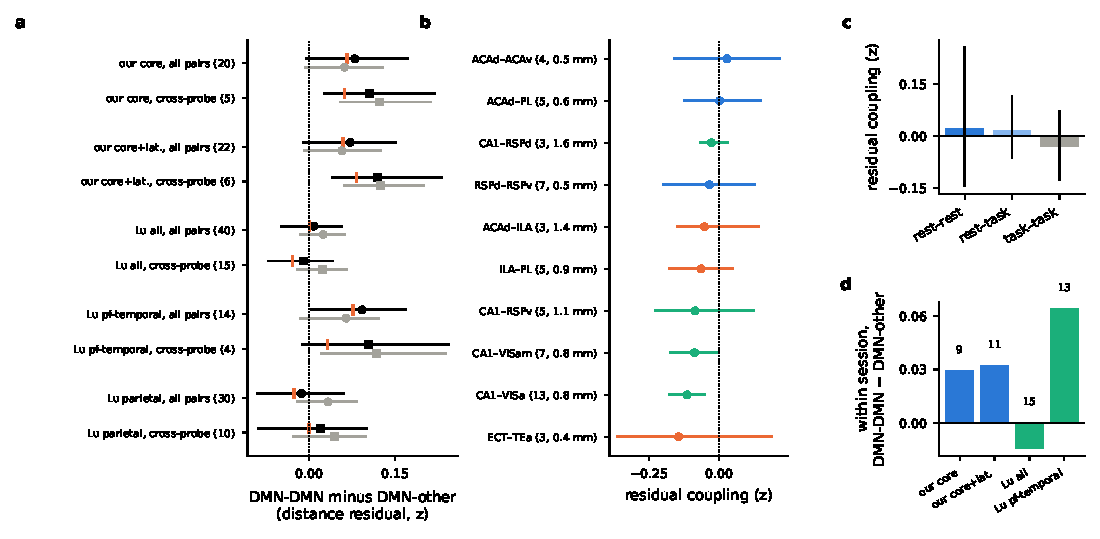
\includegraphics[width=\linewidth]{fig5_coupling_panels.pdf}
    \caption{\textbf{a} Grey-screen co-fluctuation of region signals (still bins only; wheel, lick and motion-energy regression), as residual from pairs at the same distance and probe relation. Difference DMN-DMN minus DMN-other cortical pairs for each region set, all pairs (circles) and pairs on different probes only (squares), 1 s (black) and 0.5 s (grey) bins; 95\% mouse-bootstrap CI; number of mice with a DMN-DMN pair in brackets. Orange tick: the 1 s estimate after dropping the single most coupled DMN-DMN pair. The distance baseline uses cortical and CA1 pairs only. With about 20 such contrasts, CIs that just exclude 0 would not survive correction. \textbf{b} Every DMN edge (either definition) recorded in $\geq$3 mice: mean over mice of the residual coupling, 95\% bootstrap CI; brackets give the number of mice and the median distance between the two regions. Blue: edge in both definitions; orange: our definition only; green: Lu et al. only. \textbf{c} Cross-validated rest-preference network: cortical regions ranked by grey-screen rest preference (RI) in one half of the mice (terciles), coupling measured in the other half; mean and 2.5--97.5\% range over 400 half-splits; rest--rest exceeds rest--task in 52\% of splits. \textbf{d} Within-session contrast DMN-DMN minus DMN-other, mean over mice (number of mice above bars; Lu parietal has only 2 mice and is not shown).}
    \label{fig:grey_coupling}
\end{figure}
\end{minipage}
\end{document}
